\subtop{LinkedList Darstellung}
Zur Reduzierung der Laufzeit von \union
\example{\S=\{\{1,3,5,7\},\{2,4,8\}\}, X=\{1,\dots,9\}}{
	\ \\\usetikzlibrary{positioning}
\begin{tikzpicture}[node distance=0.5cm]
\foreach \x/\y in {1/0,3/1,5/2,7/3,2/5,4/6,8/7}{
	\node(\x) at(\y,0){\x};
}
\foreach \x/\y in {3/1,5/3,7/5,4/2,8/4}
	\draw[->](\x)to node[above] {\scriptsize prev}(\y);
\foreach \x in {1,2}{
	\draw[->,loop left](\x)to node[above] {\scriptsize prev}(\x);
	\node(temp)[above=of \x,color=red]{\scriptsize\textbf{repr}};
	\draw[->,color=red](temp)--(\x);
}
\foreach \x/\y in {1/7,2/8}
	\draw[->,color=green!50!black](\x)to[out=300,in=240] node[above] {\scriptsize tail}(\y);
\end{tikzpicture}\\
}
Laufzeiten:
\begin{description}
	\item[\makeset:] $\Theta(1)$
	\item[\find:] $\Theta(n)$
	\item[\union:] $\Theta(1)$
	\item[Gesamtlaufzeit für $n-1$ \union~und $m$ \find:] $\Theta(m\cdot n)$
\end{description}
$\Rightarrow$ keine Verbesserung der Laufzeit
\topbreak
\vspace*{-2\baselineskip}
\subsection{Erweiterte LinkedList Darstellung}
\example{\S=\{\{1,3,5,7\},\{2,4,8\}\}, X=\{1,\dots,9\}}{
	\ \\\usetikzlibrary{positioning,decorations.pathreplacing}
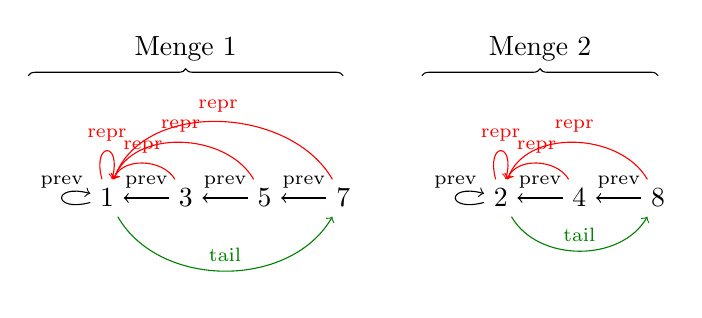
\begin{tikzpicture}[node distance=0.5cm,decoration=brace]
\foreach \x/\y in {1/0,3/1,5/2,7/3,2/5,4/6,8/7}{
	\node(\x) at(\y,0){\x};
}
\foreach \x/\y in {3/1,5/3,7/5,4/2,8/4}
	\draw[->](\x)to node[above] {\scriptsize prev}(\y);

\foreach \x in {1,2}{
	\draw[->,loop left](\x)to node[above] {\scriptsize prev}(\x);
	\draw[->,color=red,loop above](\x)to node[above] {\scriptsize repr}(\x);
}
\foreach \x/\y in {1/7,2/8}
	\draw[->,color=green!50!black](\x)to[out=300,in=240] node[above] {\scriptsize tail}(\y);
\foreach \x/\y in{3/1,5/1,7/1,4/2,8/2}{
	\draw[->,color=red](\x)to[out=120,in=70] node[above] {\scriptsize repr}(\y);
}

\draw[decorate, yshift=2ex]  (-1,1.25) -- node[above=0.4ex] {Menge 1}  (3,1.25);
\draw[decorate, yshift=2ex]  (4,1.25) -- node[above=0.4ex] {Menge 2}  (7,1.25);
\end{tikzpicture}\\
	\begin{minipage}{0.15\textwidth}
		\union($1,2$) =
	\end{minipage}\hfill
	\begin{minipage}{0.85\textwidth}
		\usetikzlibrary{positioning,decorations.pathreplacing}
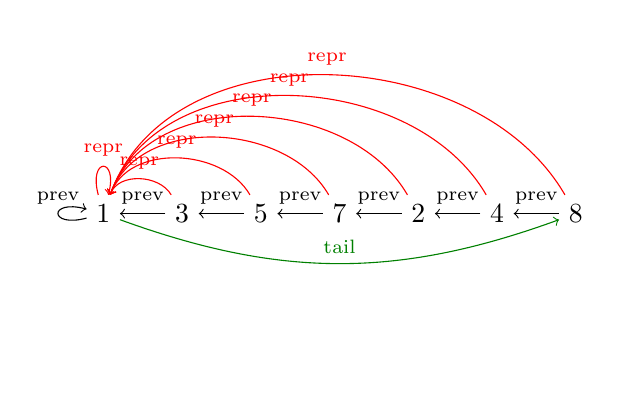
\begin{tikzpicture}[node distance=0.5cm,decoration=brace]
\foreach \x/\y in {1/0,3/1,5/2,7/3,2/4,4/5,8/6}{
	\node(\x) at(\y,0){\x};
}
\foreach \x/\y in {3/1,5/3,7/5,4/2,8/4,2/7}
	\draw[->](\x)to node[above] {\scriptsize prev}(\y);

\foreach \x in {1}{
	\draw[->,loop left](\x)to node[above] {\scriptsize prev}(\x);
	\draw[->,color=red,loop above](\x)to node[above] {\scriptsize repr}(\x);
}
\foreach \x/\y in {1/8}
	\draw[->,color=green!50!black](\x)to[out=340,in=200] node[above] {\scriptsize tail}(\y);

\foreach \x/\y in{3/1,5/1,7/1,4/1,8/1,2/1}{
	\draw[->,color=red](\x)to[out=120,in=70] node[above] {\scriptsize repr}(\y);
}
\node (phan) at (3,-2) {\phantom{a}};
\end{tikzpicture}
	\end{minipage}
}
\vspace*{-3\baselineskip}
Wenn man die Länge jeder Liste speichert und immer die kürzere Liste an die Längere hängt, wird jeder Repräsentanten-Zeiger höchstens $\floor{\log n}$-mal verändert werden.\\
Laufzeit von einer Sequenz mit $m$ Operationen (\makeset, \union, \find) liegt in $\BigO(m+n\log n)$
%TODO Tutorial
\\\\